\chapter{Sprint 2: Computing \& Storages management}
In this chapter, we focus on Sprint 2, which is dedicated to managing the computing and storage components of our application. 

The goal of this sprint is to develop and implement functionalities for effectively handling computing resources and storage systems. To ensure clarity, we will include diagrams and screenshots that depict these processes, providing a detailed understanding of the tasks accomplished during this sprint. By examining these elements in detail, we aim to demonstrate the efficient handling and optimization of computing and storage resources within our application.
\section{Analysis of Sprint 2 Requirements}
In this section, we will analyze the requirements for Sprint 2, focusing on the management of computing and storage resources. We will use use case diagrams and sequence diagrams to illustrate these requirements.


\subsection{Use case diagram of "Manage VM"}

The following figure (\hyperref[fig:use_case-manage_vm2]{Figure \ref{fig:use_case-manage_vm2}})  represents the ``Manage VM'' detailed use case.
\vspace*{2cm}
\begin{figure}[h]
  \center
%\hspace*{-0.9in}
  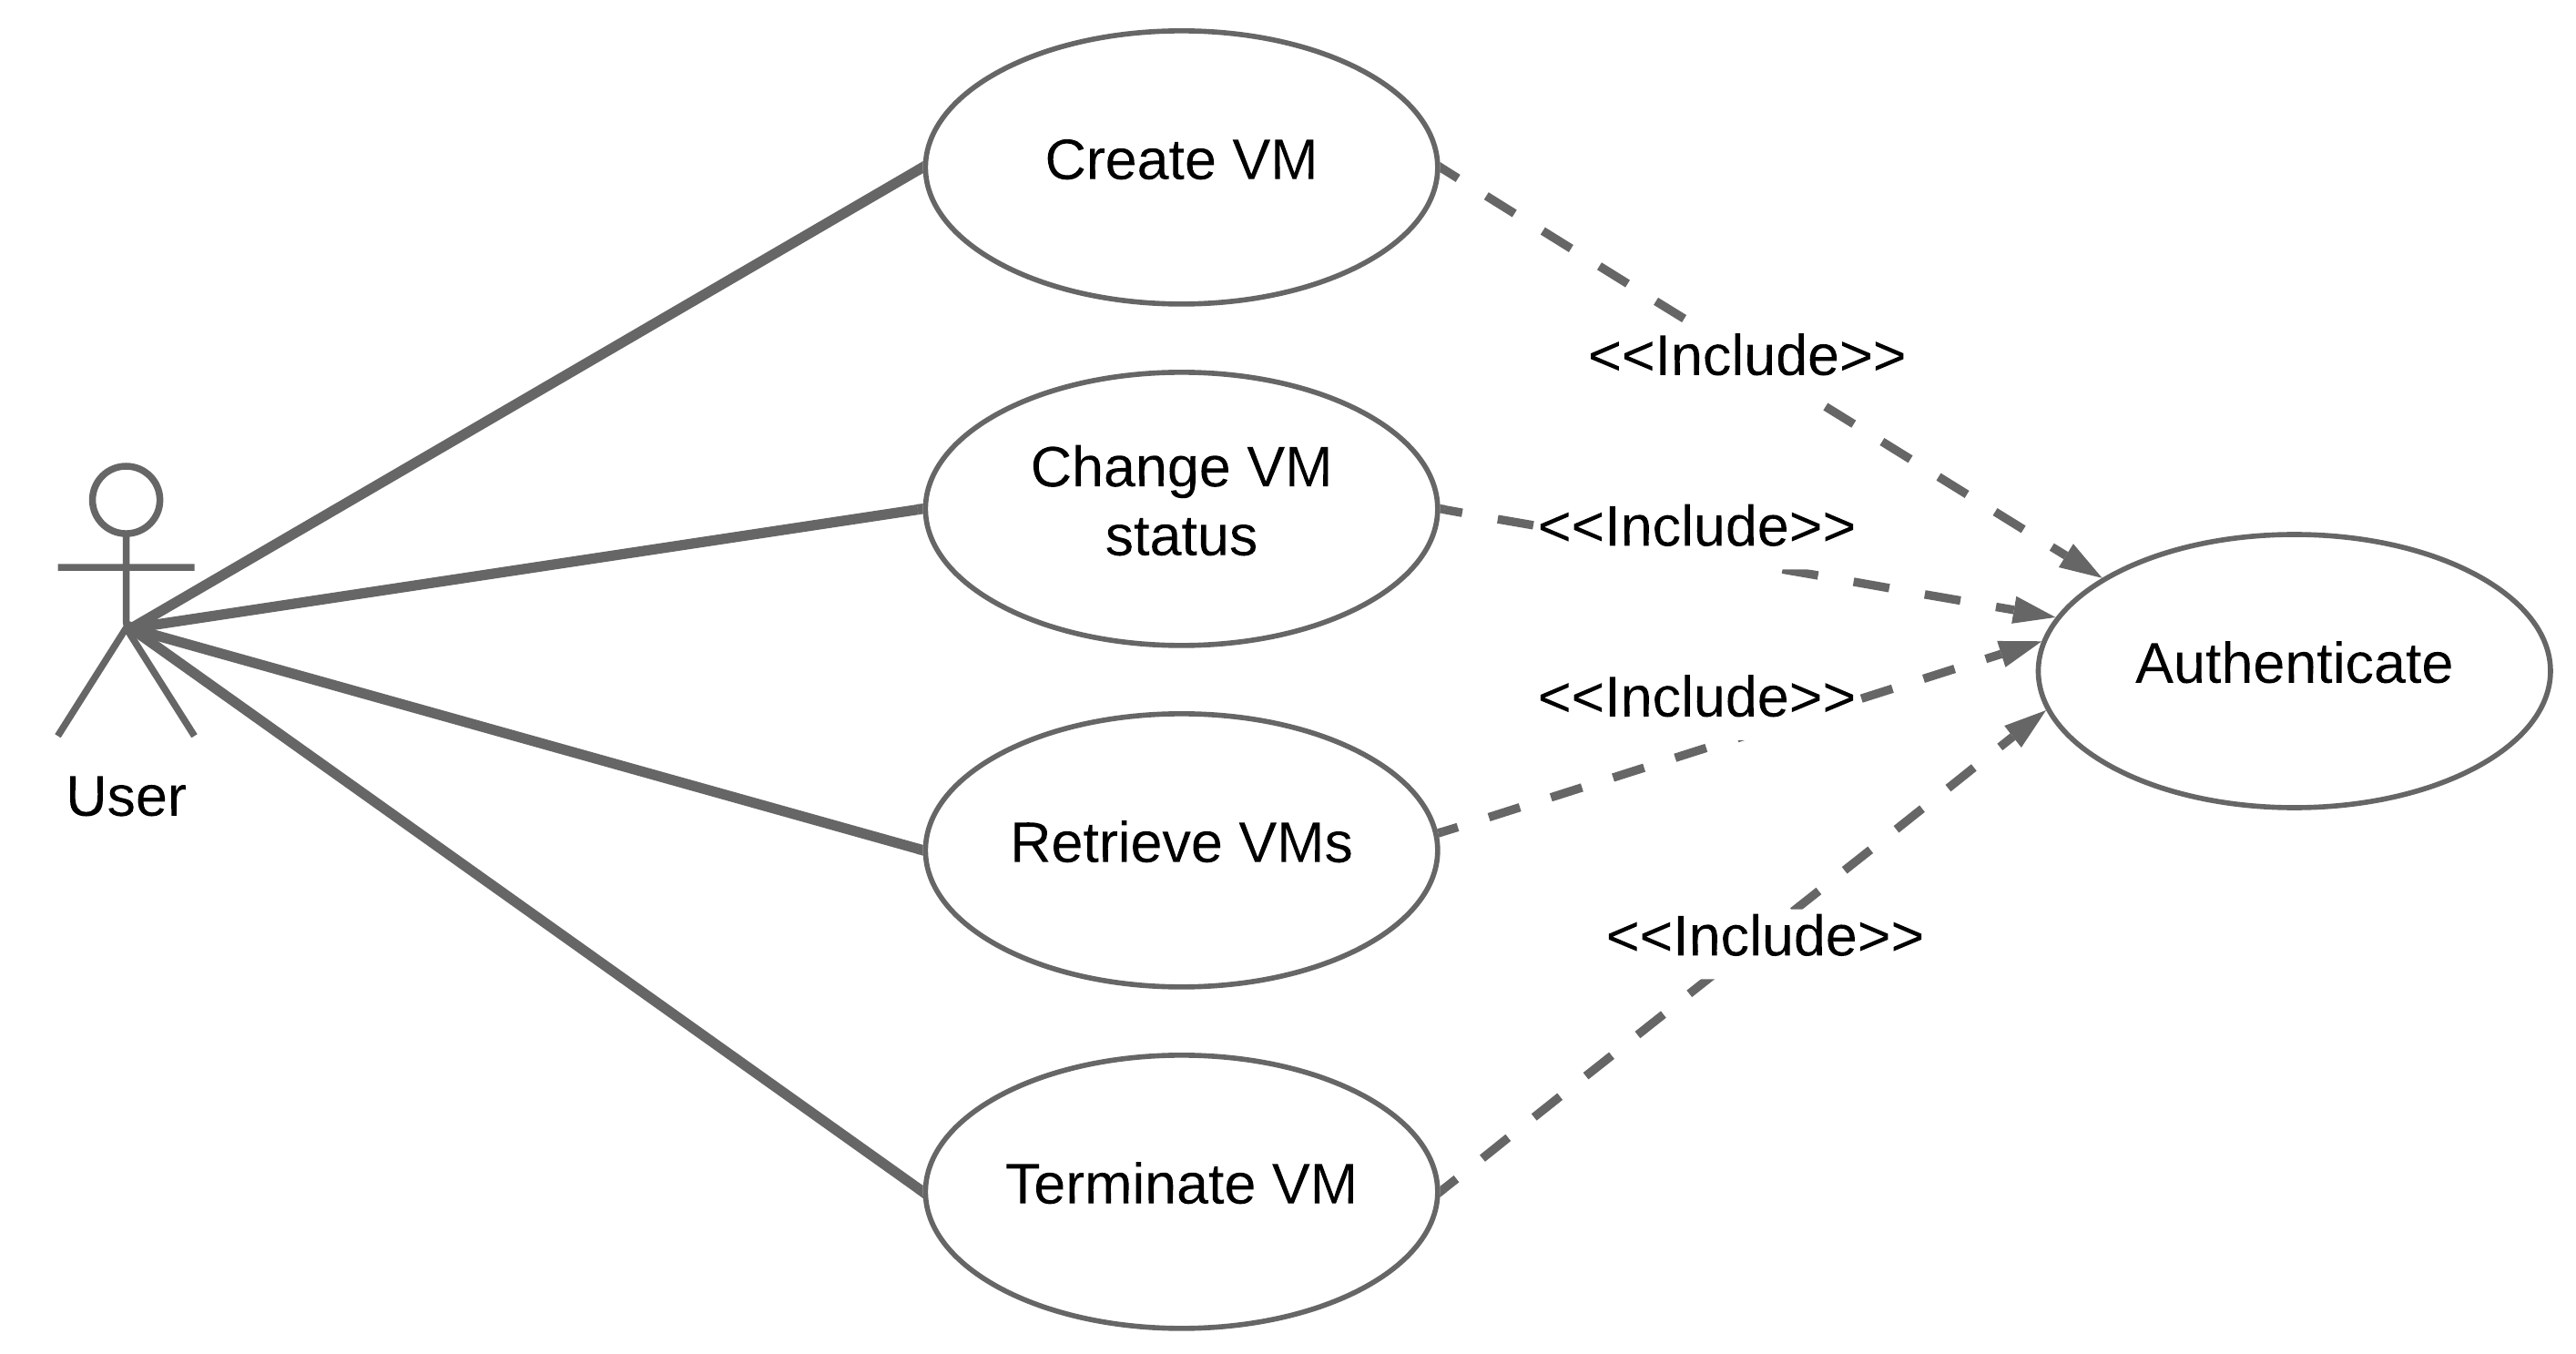
\includegraphics[width=14cm]{./chapters/sprint2/use_case-manage_vm2.png}
  \caption{Manage VM detailed use case diagram}
  \label{fig:use_case-manage_vm2}
\end{figure}
The use case diagram for instance management shows the interactions between users and the application for managing computing instances. The primary use cases include:
\begin{itemize}
  \item \textbf{Create Instance:} Users can create a new computing instance.
  \item \textbf{Start/Stop Instance:} Users can start or stop an existing instance.
  \item \textbf{Reboot Instance:} Users can reboot a running instance.
  \item \textbf{Terminate Instance:} Users can terminate an instance that is no longer needed.
\end{itemize}

\subsection{Sequence diagram of "Create Instance" use case}

The following figure (\hyperref[fig:seq-instance]{Figure \ref{fig:seq-instance}})  represents the ``Create Instance'' sequence diagram.
\begin{figure}[h]
  \center
%\hspace*{-0.9in}
  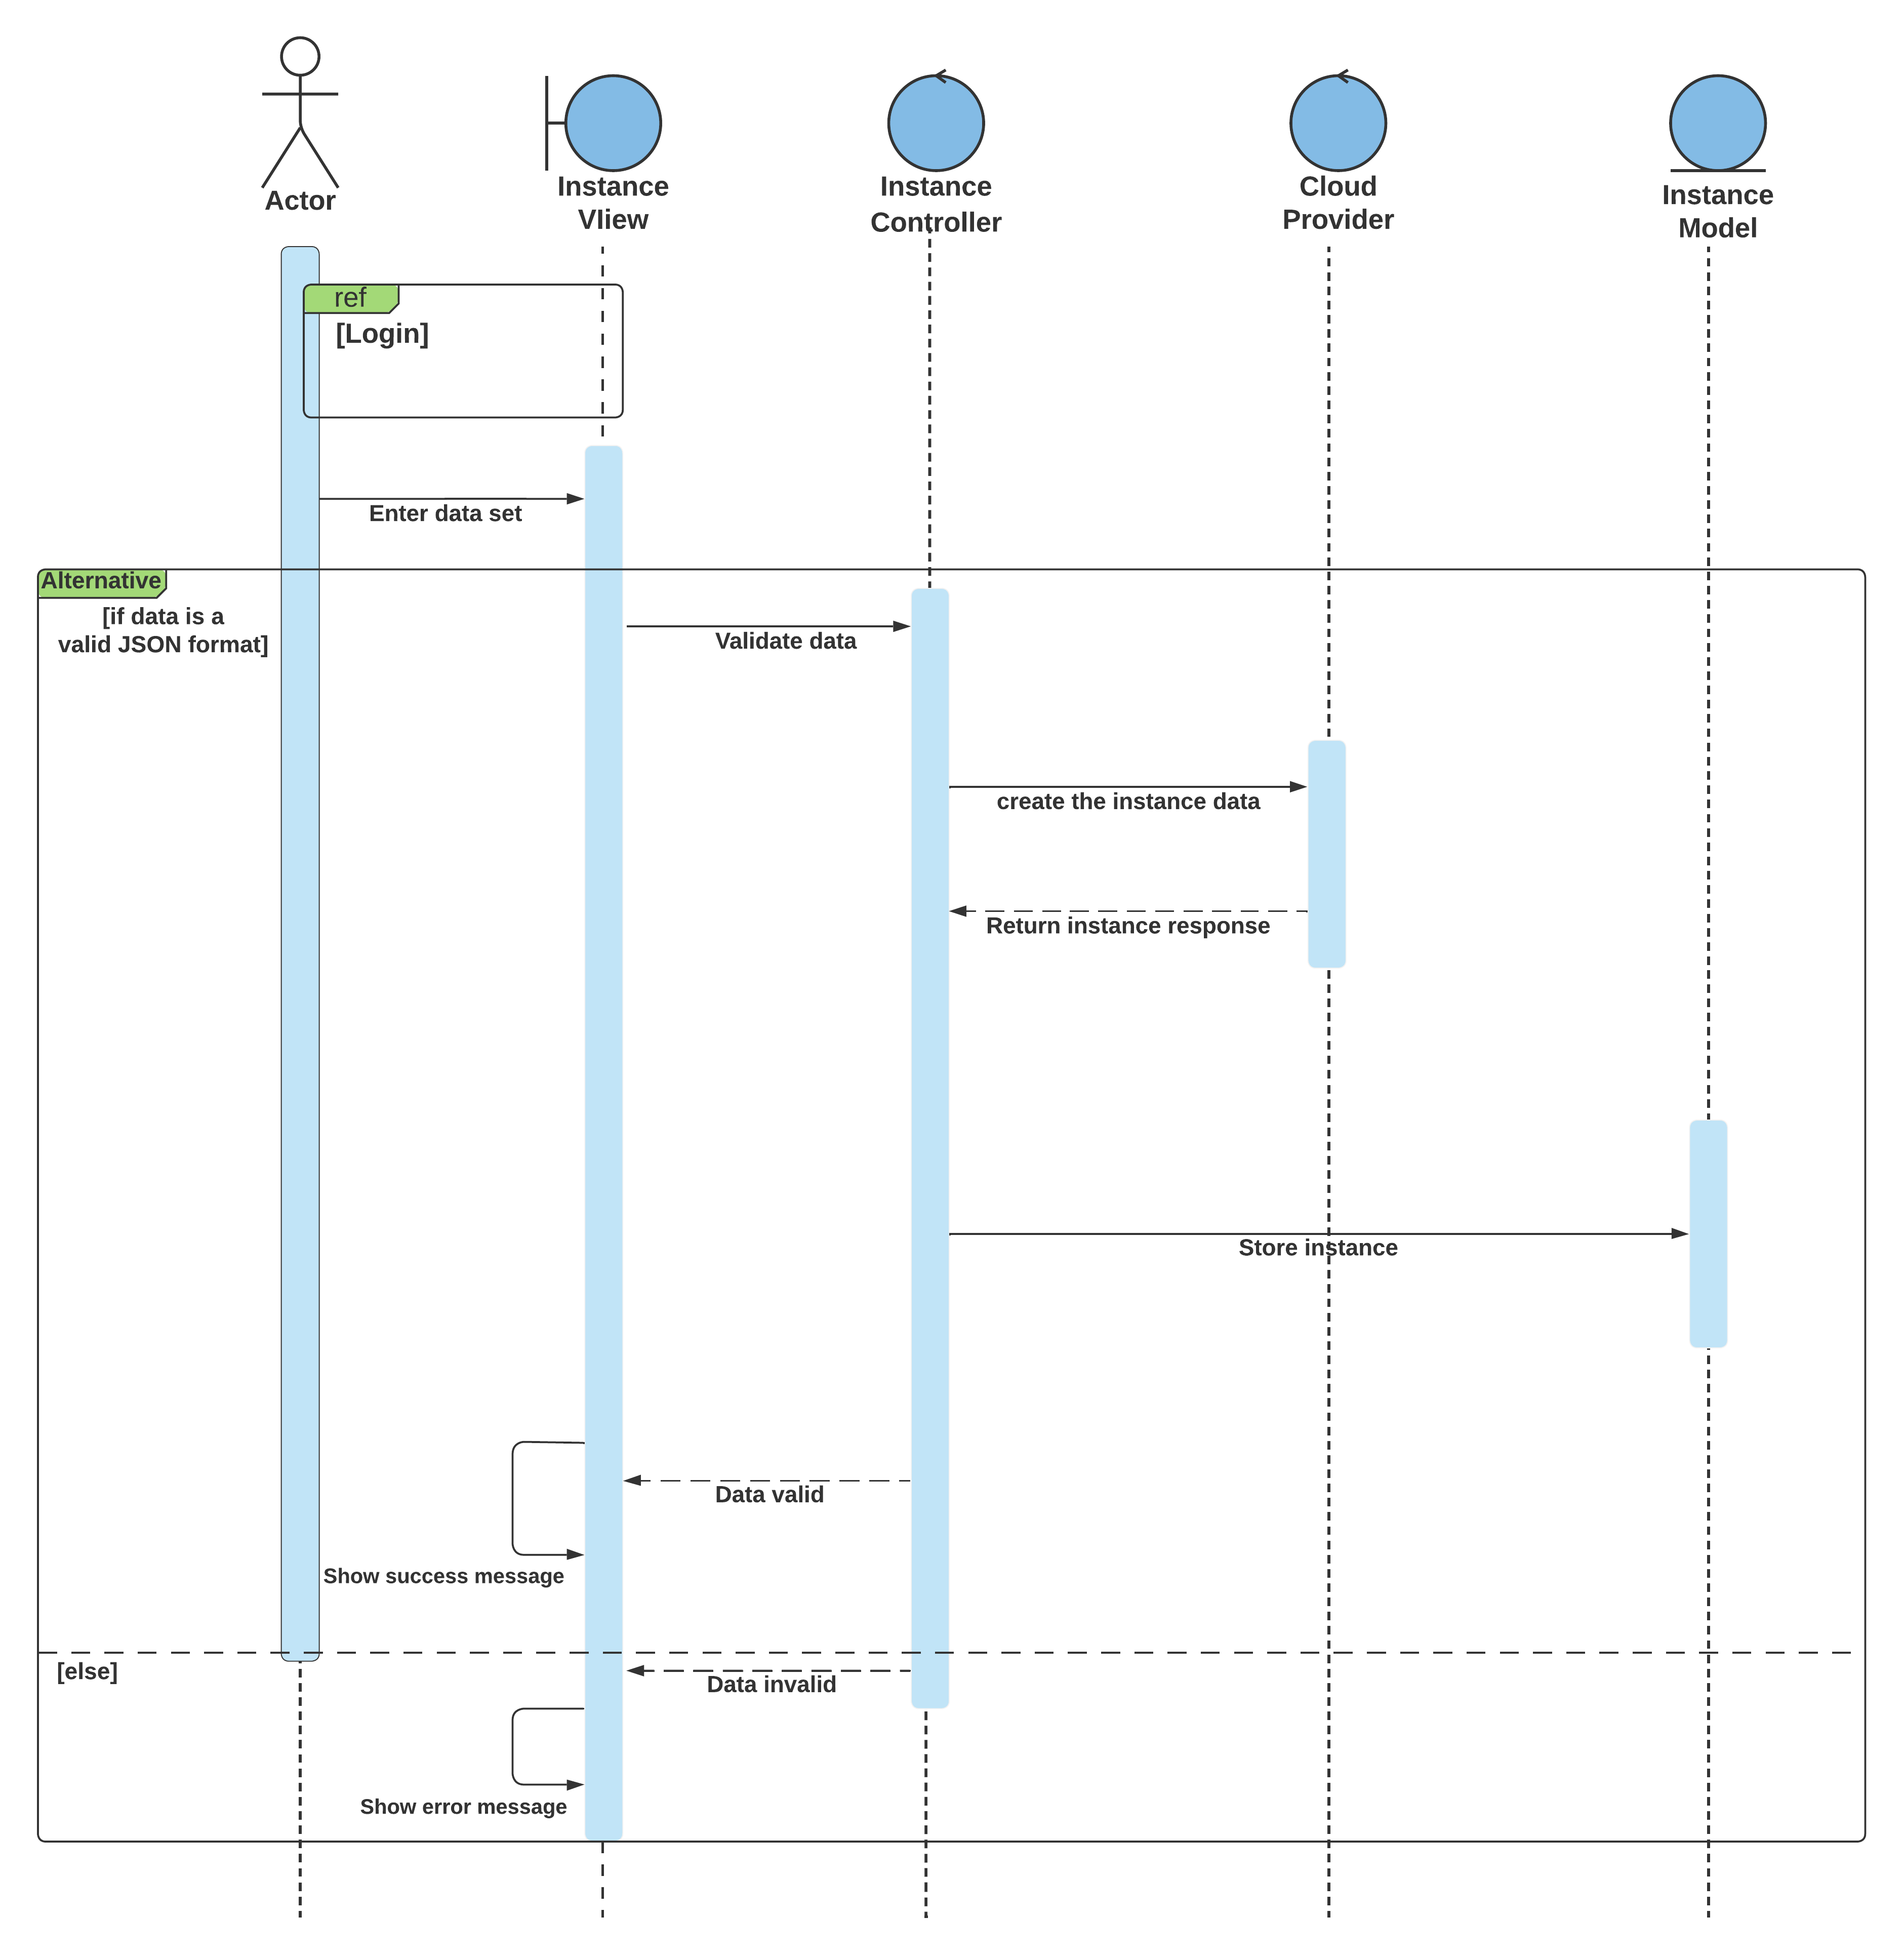
\includegraphics[width=14cm]{./chapters/sprint2/seq-instance.png}
  \caption{Sequence diagram: Create an Instance}
  \label{fig:seq-instance}
\end{figure}

\subsection{Use case diagram of "Manage Vault Secrets"}

The following figure (\hyperref[fig:use_case-manage_bucket2]{Figure \ref{fig:use_case-manage_bucket2}})  represents the ``Manage Storage'' detailed use case.
\begin{figure}[h]
  \center
%\hspace*{-0.9in}
  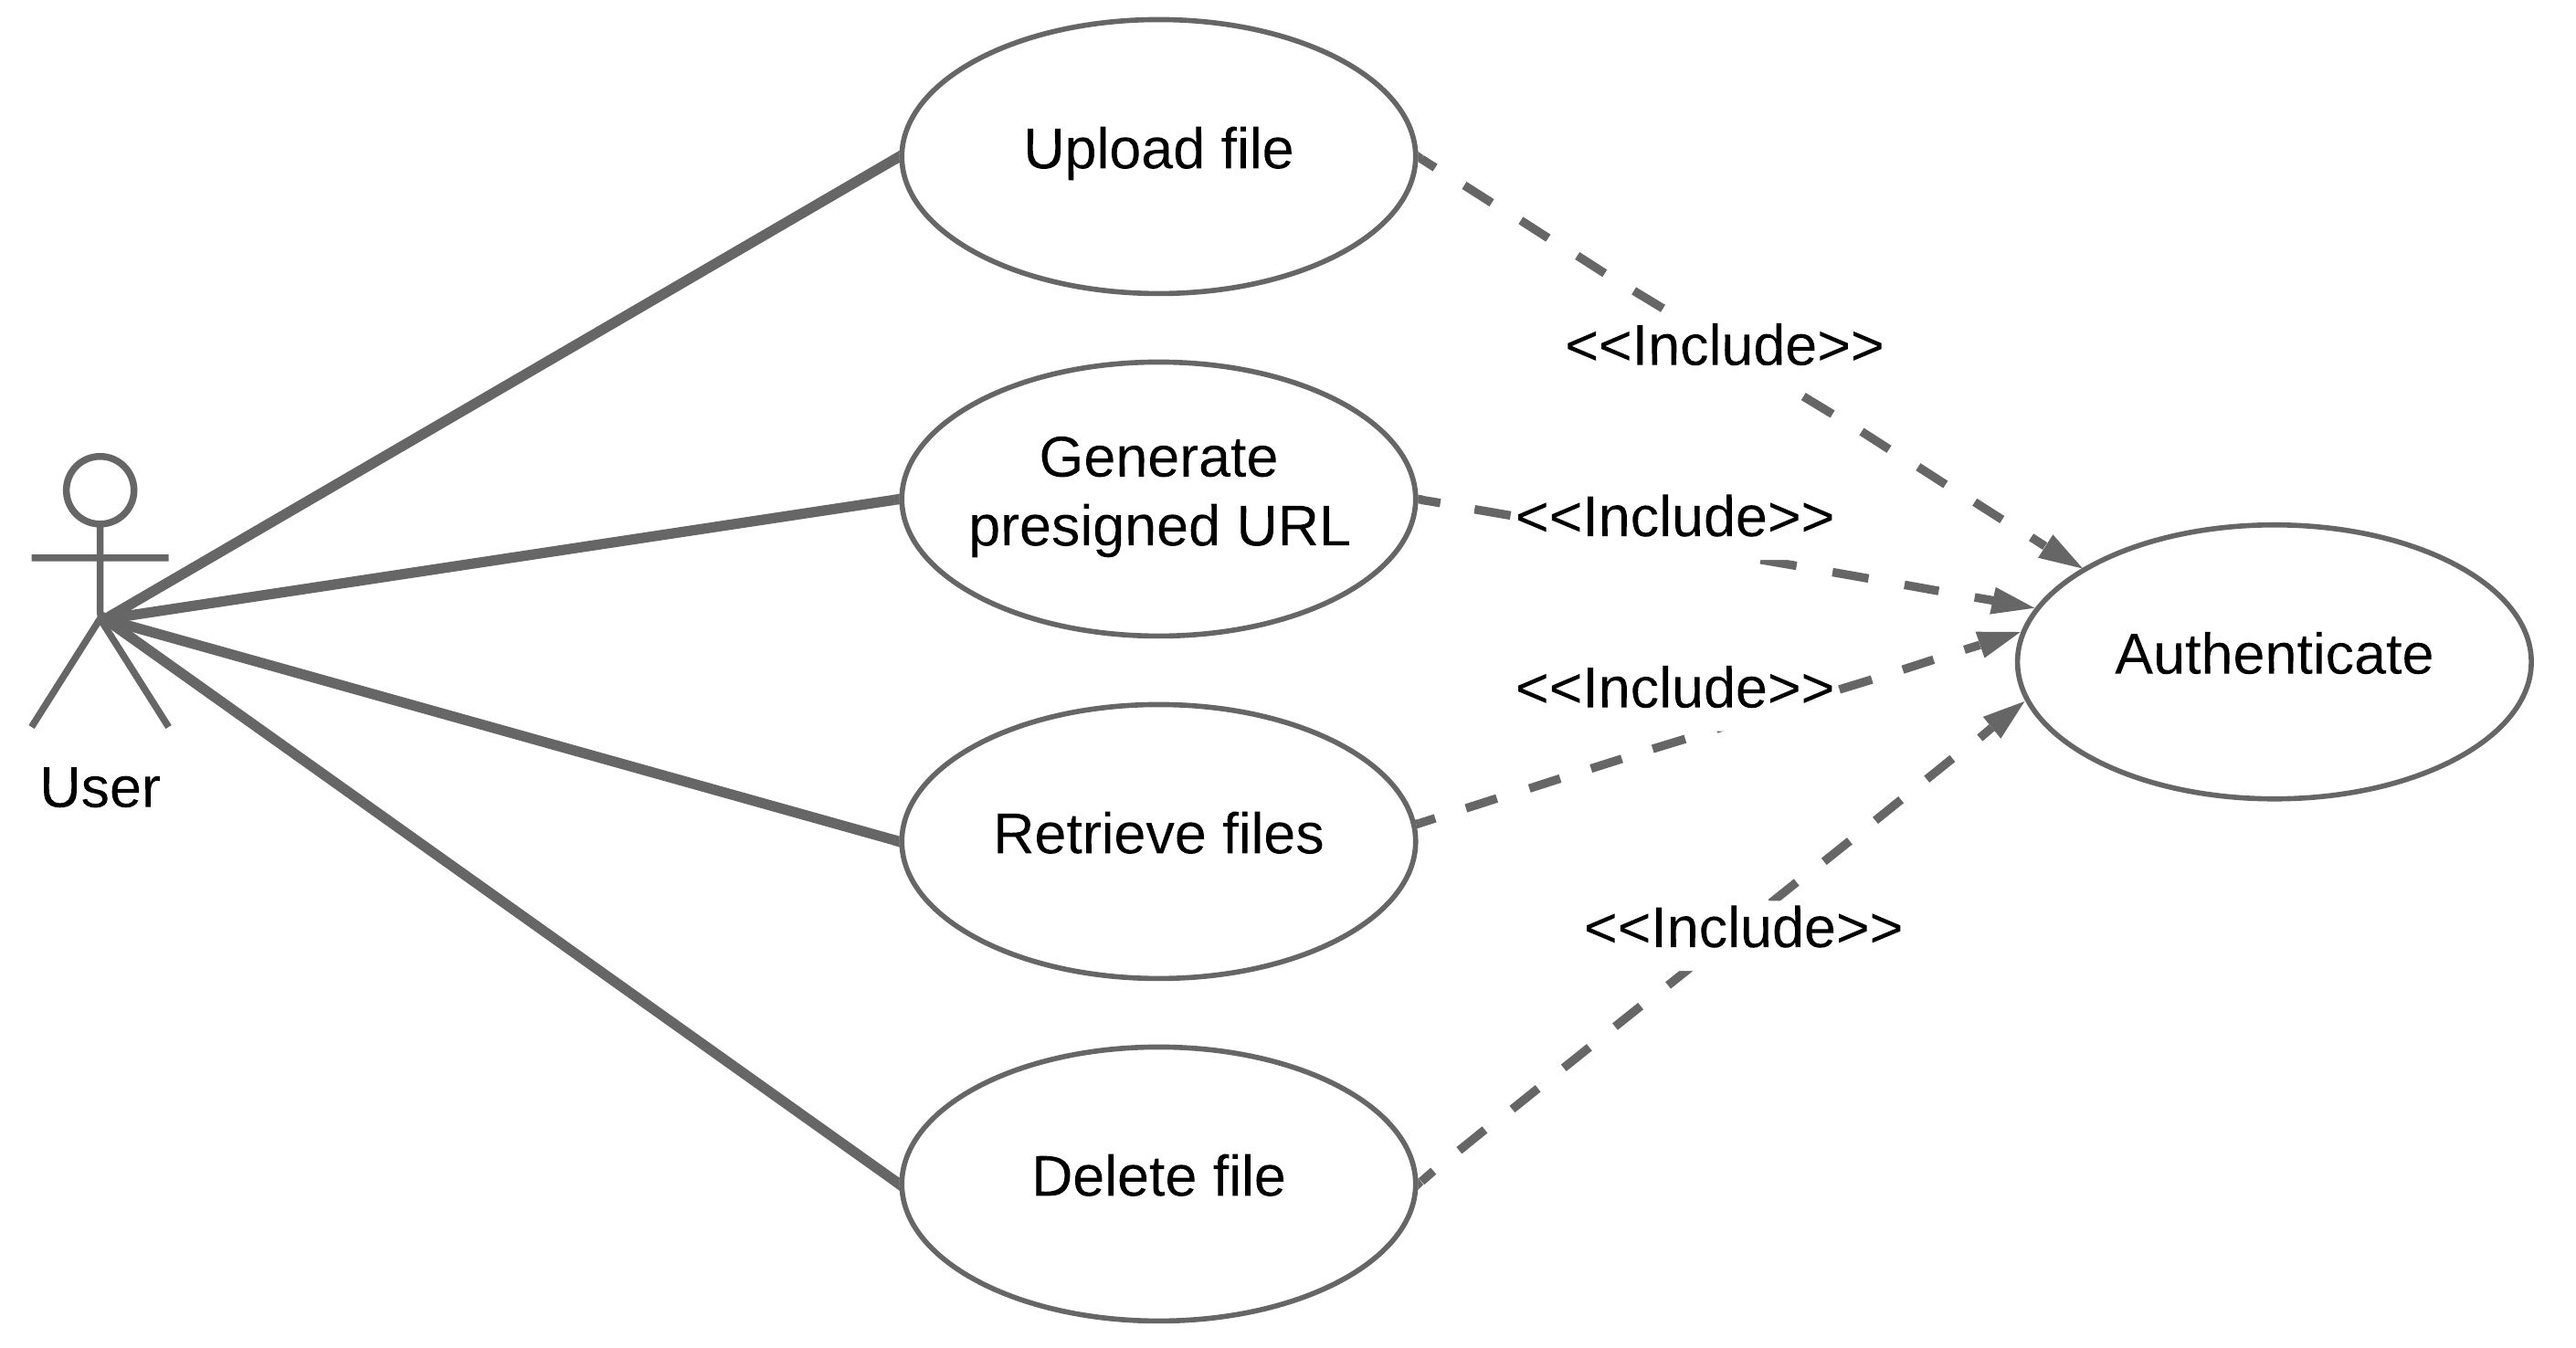
\includegraphics[width=14cm]{./chapters/sprint2/use_case-manage_bucket2.png}
  \caption{Manage Storage detailed use case diagram}
  \label{fig:use_case-manage_bucket2}
\end{figure}

The use case diagram for storage management illustrates how users interact with the application to manage storage resources. The main use cases include:

\begin{itemize}
  \item \textbf{Upload File:} Users can upload files to the cloud providers storage service.
  \item \textbf{Delete File:} Users can delete files.
  \item \textbf{Generate Presigned URL:} Users can generate presigned URLs for secure access to files.
\end{itemize}

\subsection{Sequence diagram of "Upload Storage" use case}

The following figure (\hyperref[fig:seq-instance]{Figure \ref{fig:seq-instance}})  represents the ``Create Instance'' sequence diagram.
\begin{figure}[h]
  \center
%\hspace*{-0.9in}
  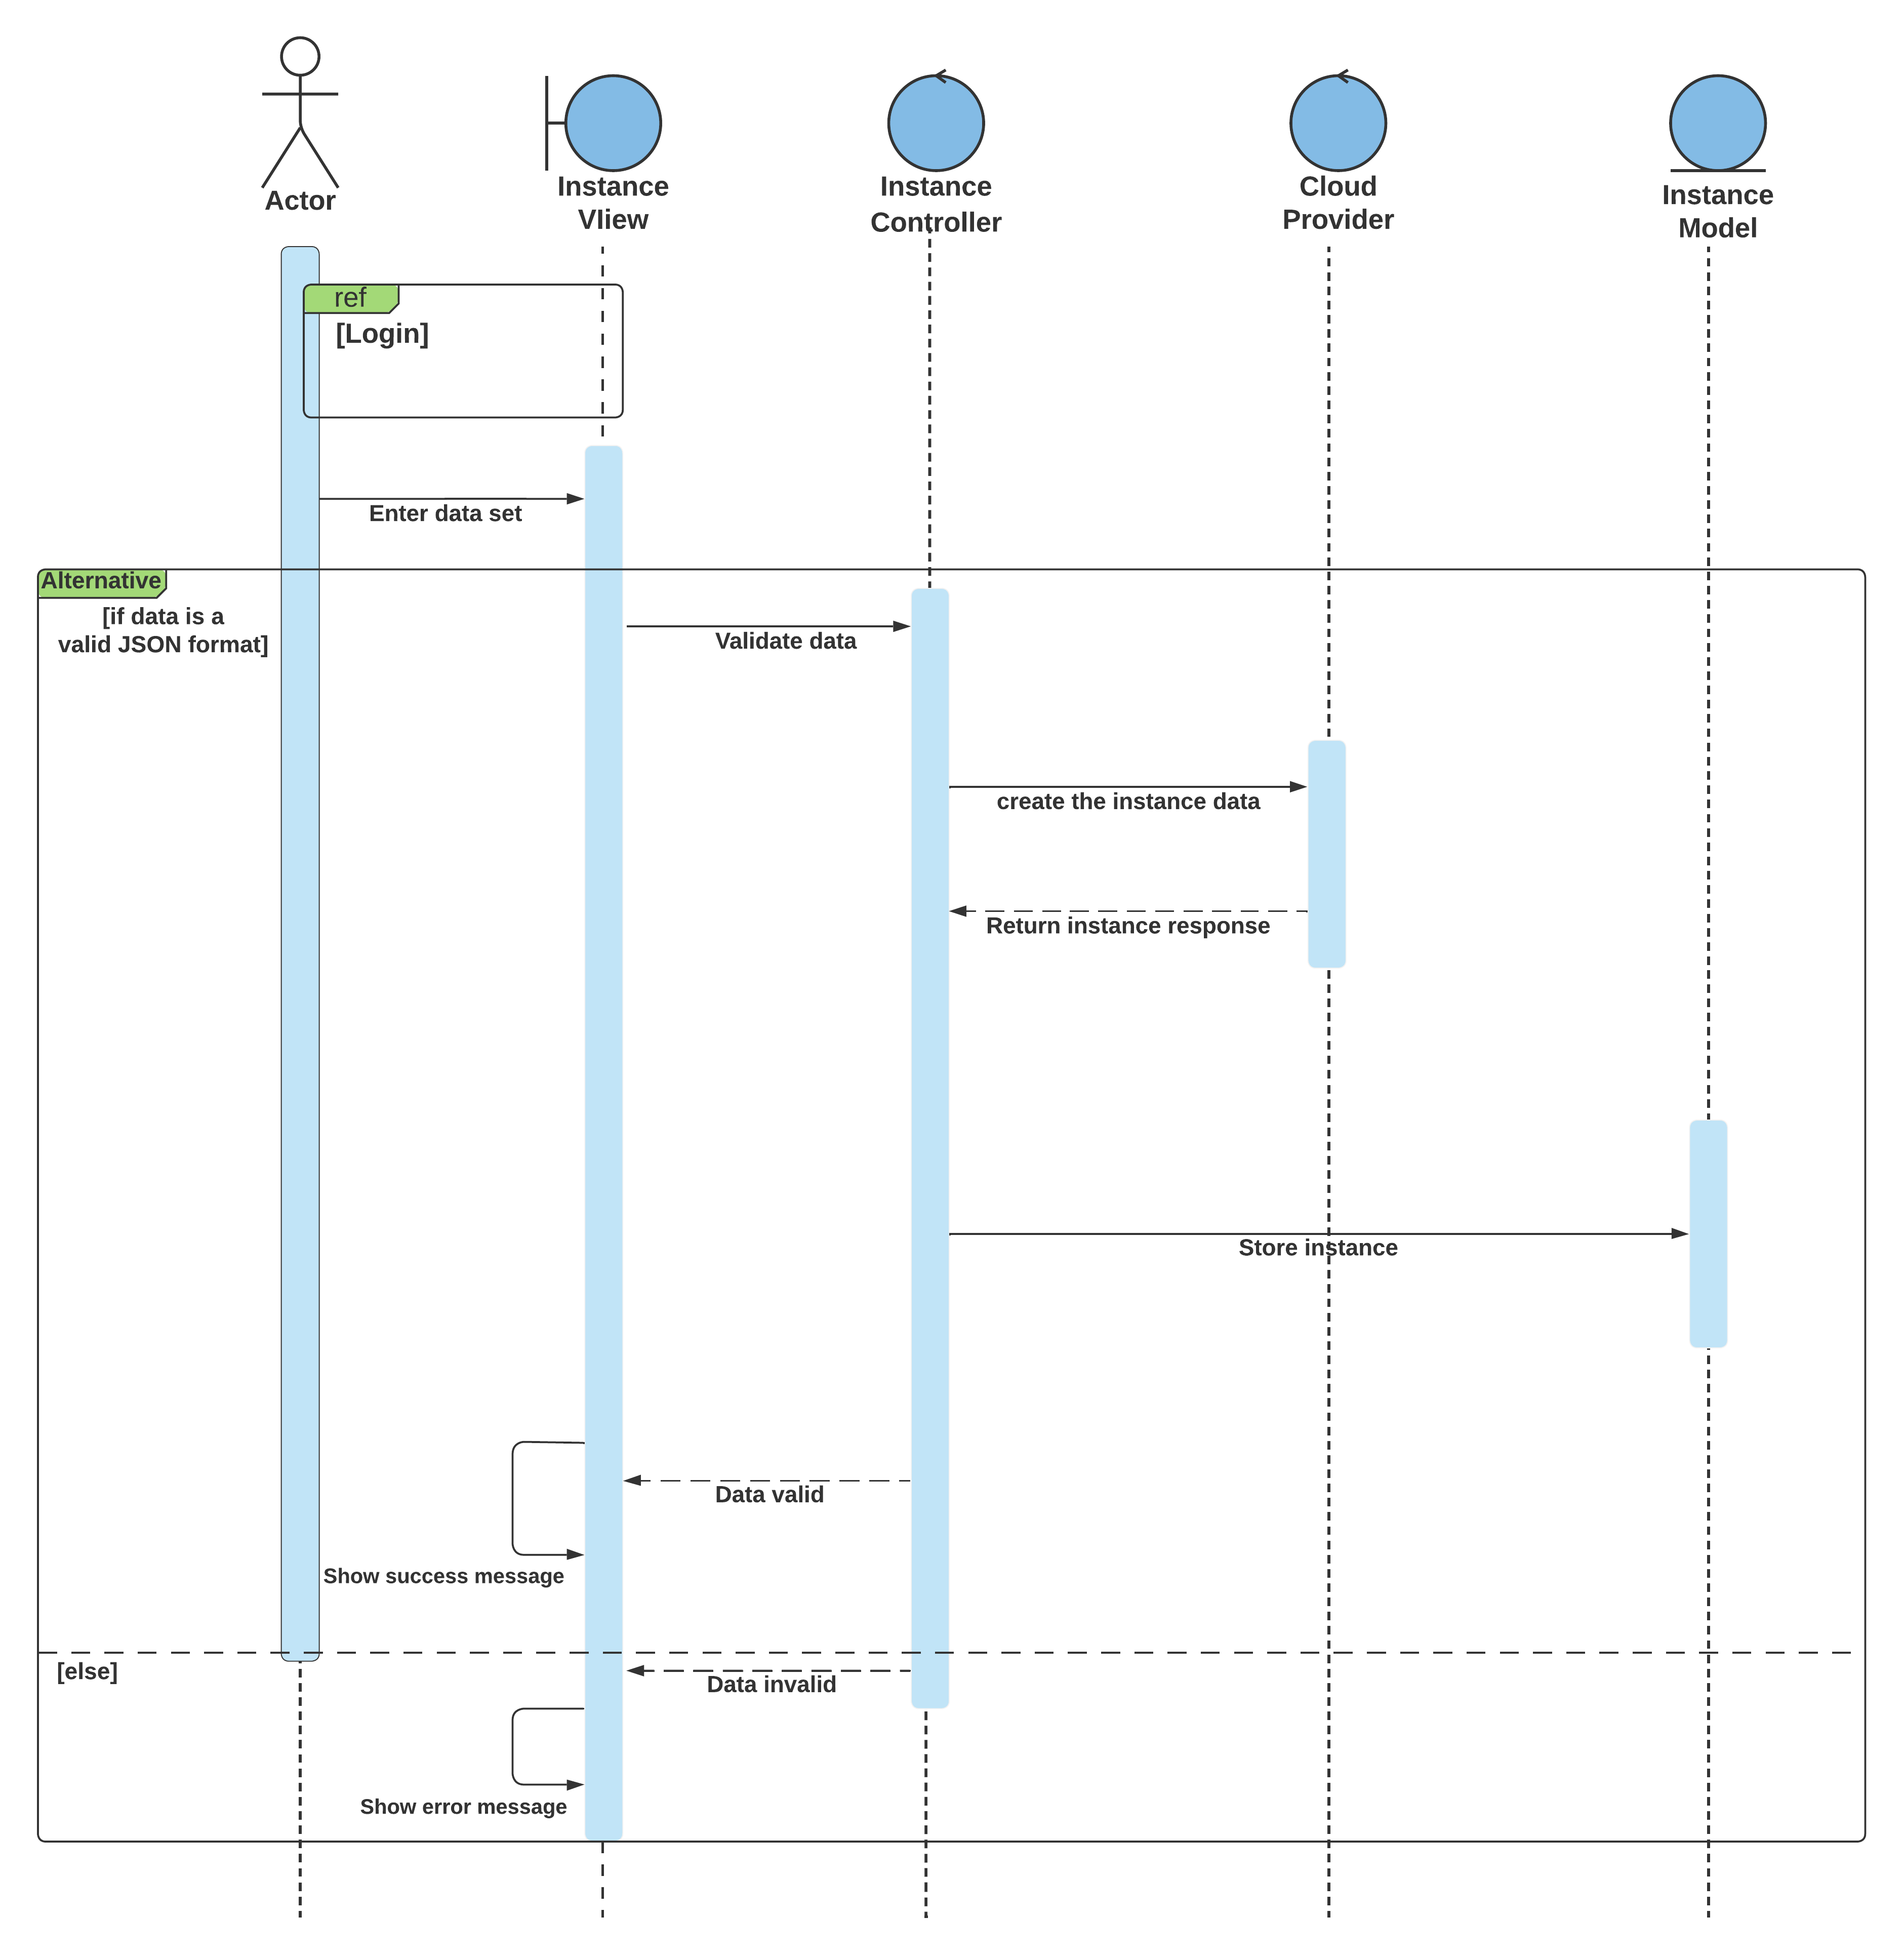
\includegraphics[width=14cm]{./chapters/sprint2/seq-instance.png}
  \caption{Sequence diagram: Upload Storage}
  \label{fig:seq-instance}
\end{figure}

\subsection{Interfaces}
In this section, we will provide some screenshots of our application interfaces. These screenshots will illustrate the various functionalities and processes related to user management as part of Sprint 1, as well as managing vault secrets. 

The following figure (\hyperref[fig:instances]{Figure \ref{fig:instances}})  depicts the instance page of our application.
\begin{figure}[h]
  \center
%\hspace*{-0.9in}
  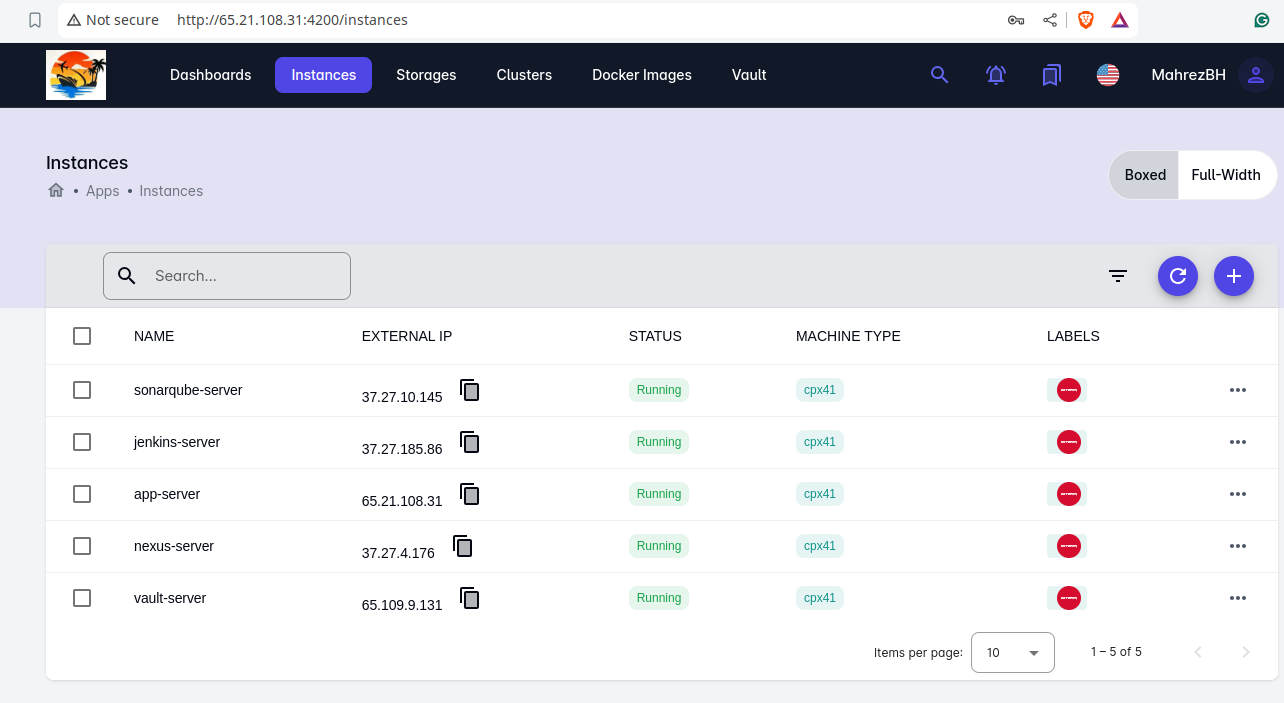
\includegraphics[width=13cm]{./chapters/sprint2/instances.png}
  \caption{Ilef instances page}
  \label{fig:instances}
\end{figure}


The following figure (\hyperref[fig:storages]{Figure \ref{fig:storages}}) represents the storages interface of our application.

\begin{figure}[h]
  \center
%\hspace*{-0.9in}
  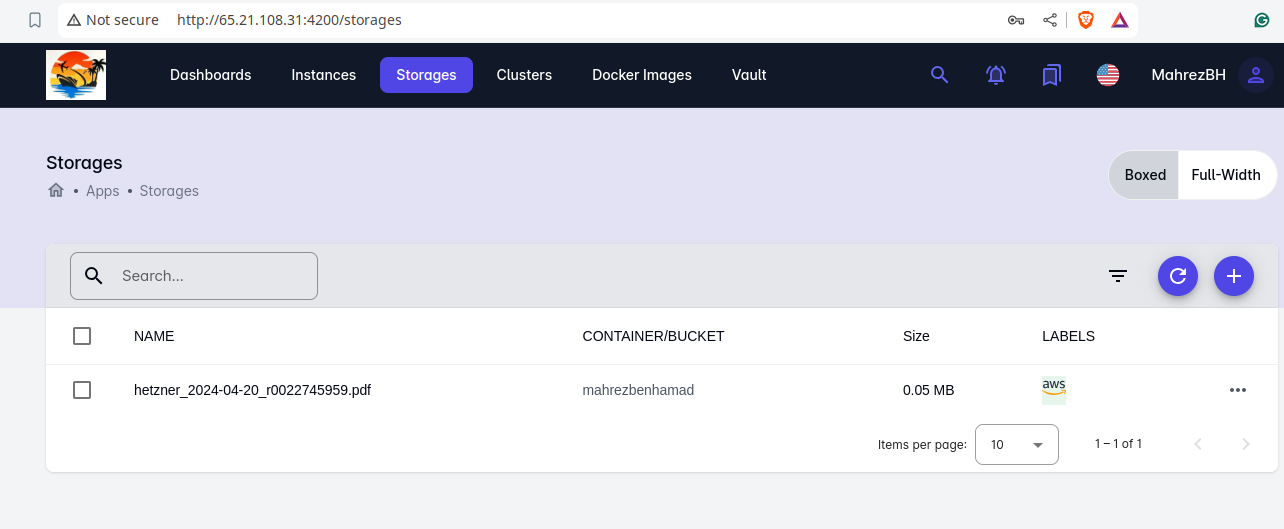
\includegraphics[width=15cm]{./chapters/sprint2/storages.png}
  \caption{Ilef storages page}
  \label{fig:storages}
\end{figure}

\vspace*{15cm}

\section*{Conclusion}
In this chapter, we analyzed the requirements for Sprint 2, focusing on computing and storage management. We utilized use case and sequence diagrams to illustrate the interactions and workflows for instance and storage management. These diagrams provided a clear understanding of the functionalities and processes implemented during this sprint.

By visualizing these requirements, we ensured that development and implementation are well-defined and aligned with our project objectives. This examination optimizes the handling and utilization of computing and storage resources, enhancing the efficiency and effectiveness of our system and contributing to the project's overall success.